\documentclass[a4paper]{article}
\usepackage[utf8]{inputenc}
\usepackage[T1]{fontenc}
\usepackage{lmodern}
\usepackage{listings}
\usepackage{graphicx}
\usepackage{dirtree}
\usepackage{caption}
\usepackage{subcaption}
\usepackage{float}
\usepackage[english]{babel}
\usepackage[margin=1.1in]{geometry}
\title{HiBoP Database Manager \\ User Manual}
\author{\textsc{BONTEMPS Benjamin} \\ \textsc{GANNERIE Adrien}}
\lstset{
	frame = single,
	basicstyle = \footnotesize\ttfamily
}

\begin{document}
\maketitle
\begin{abstract}
This document is the user manual of the Human Intracranial Brain Observation Player Database Manager (HiBoP DBM). The HiBoP DBM is being developed by the Centre de Recherche en Neurosciences de Lyon (CRNL) to manage the local iEEG database and help create projects for HiBoP, as well as converting parts of the database to BIDS format.
\end{abstract}
\tableofcontents
\section{HiBoP Database Manager}\label{bddmanager}
\paragraph{} The HiBoP Database Manager (DB Manager) can be used to manage the anatomical and functional databases (as long as they respect the hierarchy described in appendix \ref{bddhierarchy}), create HiBoP projects using huge amounts of data in no time or convert the databases to the Brain Imaging Data Structure (BIDS) format\footnote{More information about BIDS can be found at http://bids.neuroimaging.io/}. The main window (Figure \ref{dbManagerMain}) of the DB Manager has two main columns. The left column allows you to select patients to visualize their anatomical data, the right column is for functional data.
\begin{figure}[H]
\begin{center}
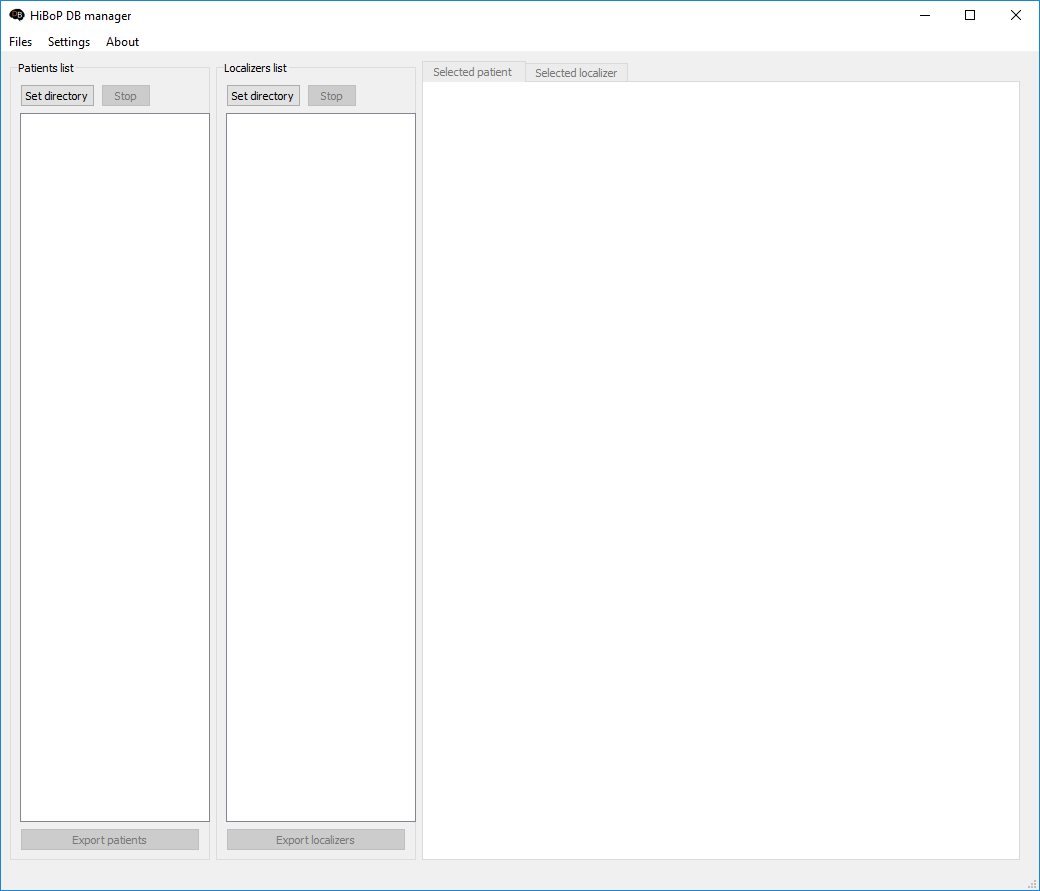
\includegraphics[scale=0.3]{DBManagerMain.png}
\end{center}
\caption{\label{dbManagerMain}Main window of the DB Manager}
\end{figure}
\subsection{Anatomical data}
\paragraph{} Click « Set Directory » in the first column to select the folder containing the anatomical database. After choosing a folder, patients found within that database will appear in the first column. Selecting one patient will display in the middle panel (Figure \ref{dbManagerPatient}) a list of files types and their status (present in green or absent in red). Some of the files can be visualized or opened directly from that interface. The display allows the user to quickly browse through patients and identify missing files.
\begin{figure}[H]
\begin{center}
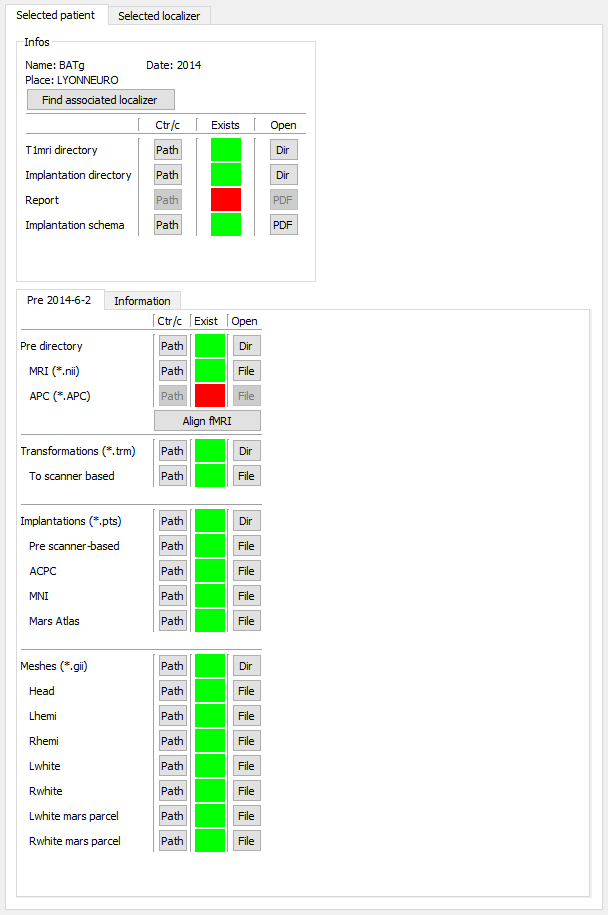
\includegraphics[scale=0.5]{DBManagerPatient.png}
\end{center}
\caption{\label{dbManagerPatient}Patient panel}
\end{figure}
\subsection{Functional data}
\paragraph{} Click « Set Directory » in the second column to select the folder containing the functional database. Once loaded, the database can be inspected patient by patient in a way similar to anatomical data (Figure \ref{dbManagerLoca}). Missing files can be quickly identified this way.
\begin{figure}[H]
\begin{center}
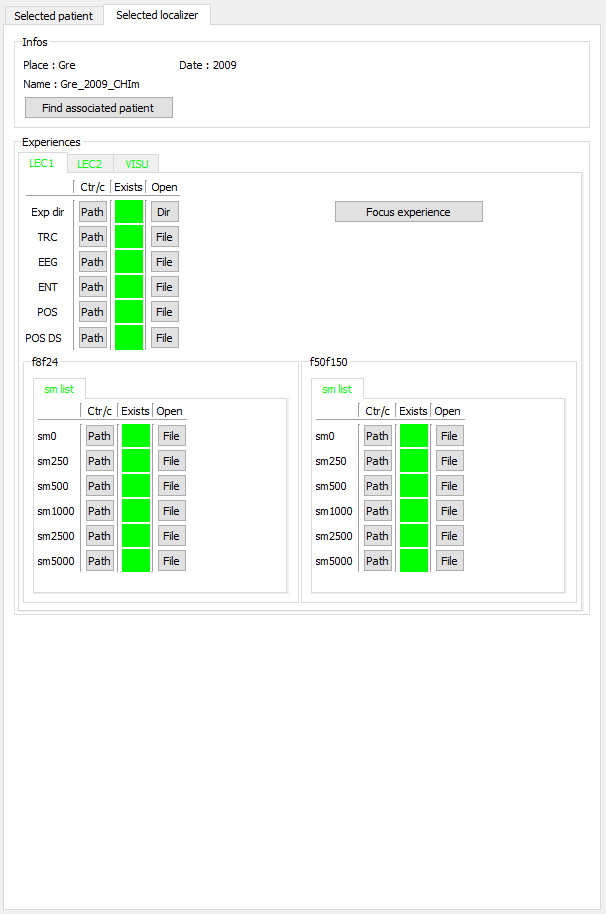
\includegraphics[scale=0.5]{DBManagerLoca.png}
\end{center}
\caption{\label{dbManagerLoca}Localizer (iEEG data) panel}
\end{figure}
\subsection{Exporting data}
\paragraph{} A panel in the right part (Figure \ref{dbManagerFilters}) of the window allows the user to filter patients. By checking boxes, you can quickly identify patients matching certain criteria (e.g. all patients with task LEC2, with gamma envelopes and anatomical MRIs).
\begin{figure}[H]
\begin{center}
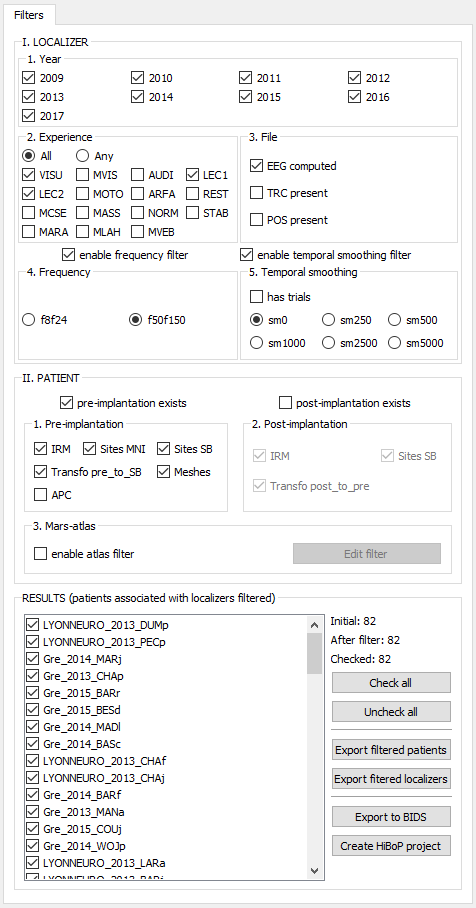
\includegraphics[scale=0.5]{DBManagerFilters.png}
\end{center}
\caption{\label{dbManagerFilters}Export panel}
\end{figure}
\paragraph{} You can filter using the following parameters:
\begin{itemize}
\item \textbf{Year}: Choose patients of specific years.
\item \textbf{Experience}: Choose patients based on the tasks they performed.
\item \textbf{Files}: Choose patients with specific functional files (.TRC, .eeg, .pos)
\item \textbf{Frequency}: Choose patients with processed data using specific frequency range\footnote{Hilbert transform: f8f24 combines the alpha and beta frequency bands, f50f150 corresponds to the gamma band.}.
\item \textbf{Smoothing}: Choose patients with data with a specific temporal smoothing.
\item \textbf{Patient}: Choose patients with specific anatomical criteria: pre implantation files, post implantation files, presence of a site in a specific Mars Atlas area etc.
\end{itemize}
\paragraph{} Once you have selected the patients you want to study (using the boxes next to their names; a red name means this patient does not match one of the parameters you chose), you can create a HiBoP project using these patients, export these patients to BIDS format, export the anatomical files (section \ref{exportAnatomical}) or the functional files (section \ref{exportFunctional}) to another folder.
\subsubsection{Anatomical data}\label{exportAnatomical}
\paragraph{} If you click on the "Export patients" button, you will see the window presented in figure \ref{dbManagerExportPatient}. There you can choose which files you want to export (MRI, Implantations, Meshes etc.) or you can export the whole database (even files which are not recognized by the database manager). When you are ready to export, click on the "Start export" button and select the folder that will be containing your exported anatomical database. You can cancel the export at any time.
\begin{figure}[H]
\begin{center}
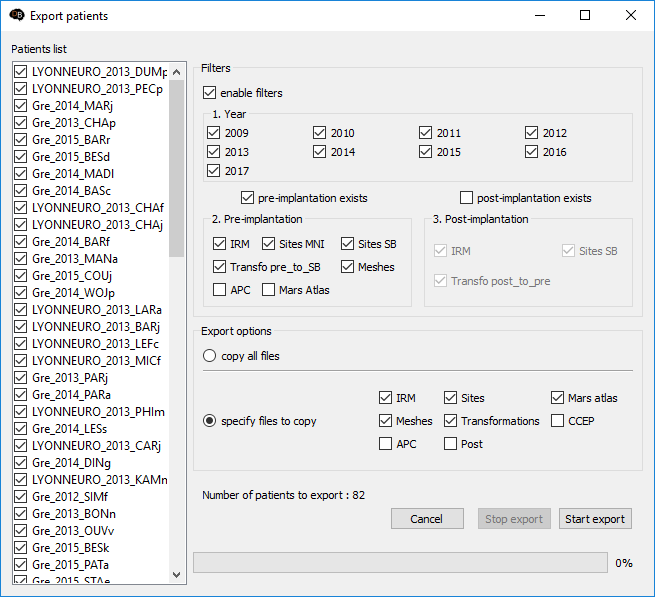
\includegraphics[scale=0.5]{ExportPatient.png}
\end{center}
\caption{\label{dbManagerExportPatient}Export patients window}
\end{figure}
\subsubsection{Functional data}\label{exportFunctional}
\paragraph{} Exporting functional data is very similar to exporting anatomical data (Figure \ref{dbManagerExportLoca}).
\begin{figure}[H]
\begin{center}
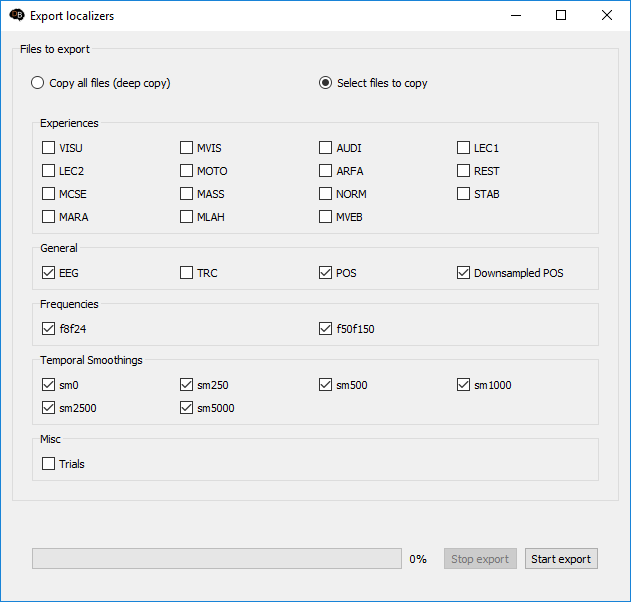
\includegraphics[scale=0.5]{ExportLoca.png}
\end{center}
\caption{\label{dbManagerExportLoca}Export localizers window}
\end{figure}
\subsection{Resources files}
\paragraph{} A folder called "resources" is present next to the executable of the DB Manager. It contains useful files for the DB Manager to work. These files can either be edited using a text editor or, for some files only, you can edit them safely using Settings/Edit experiences sub-menu. They contain:
\begin{itemize}
\item \textbf{broadman\_areas.txt}: links between the name of a broadman area and its respective index
\item \textbf{corr\_nomenclature.txt}: links between the names of the same patient in the anatomical database (right) and in the functional database (left)
\item \textbf{Downsamplings.txt}: list of possible values for the downsamplings
\item \textbf{Experiences.txt}: list of experiences to find in the functional database
\item \textbf{Frequencies.txt}: list of possible values for frequency ranges
\item \textbf{localizers.tsv}: metadata for the localizers used to convert the database to BIDS
\item \textbf{mars\_atlas\_index.csv}: links between the name of a mars atlas area and its respective index
\item \textbf{TemporalSmoothings.txt}: list of possible values for the temporal smoothings
\item \textbf{Years.txt}: list of possible values for the years
\item \textbf{Images localizers}: this folder contains illustrations for the localizers (these images are exported into the HiBoP project created with the DB Manager)
\item \textbf{Protocols}: this folder contains .prov files readable by HiBoP to describe the localizers (these protocol files are exported into the HiBoP project created with the DB Manager)
\end{itemize}
\section{HiBoP Database Hierarchy}\label{bddhierarchy}
\paragraph{} In order to use HiBoP and the DB Manager with automatic loading of patients, a specific hierarchy of the database must be respected. There is a specific hierarchy for the anatomical database (usable in both HiBoP and the Database Manager) and for the functional database (usable only in the Database Manager). These are presented in the following sections. Note that BIDS format will be supported in a near future.
\subsection{Anatomical database}
\begin{figure}[H]
\framebox[\textwidth]{%
\begin{minipage}{0.9\textwidth}
\dirtree{%
	.1 Database/.
	.2 <PATIENT>/.
	.3 implantation/.
	.4 <PATIENT>.pts.
	.4 <PATIENT>\_MNI.pts.
	.4 <PATIENT>\_ACPC.pts.
	.4 <PATIENT>.csv.
	.3 t1mri/.
	.4 T1pre\_<DATEFULL>/.
	.5 <PATIENT>.nii.
	.5 registration/.
	.6 RawT1-<PATIENT>\_T1pre\_<DATEFULL>\\\_TO\_Scanner\_Based.trm.
	.5 default\_analysis/.
	.6 segmentation/.
	.7 mesh/.
	.8 <PATIENT>\_Lhemi.gii.
	.8 <PATIENT>\_Rhemi.gii.
	.8 <PATIENT>\_Lwhite.gii.
	.8 <PATIENT>\_Rwhite.gii.
	.8 surface\_analysis/.
	.9 <PATIENT>\_Lwhite\_parcels\\\_marsAtlas.gii.
	.9 <PATIENT>\_Rwhite\_parcels\\\_marsAtlas.gii.
	.4 T1post\_<DATEFULL>/.
	.5 <PATIENT>.nii.
	.5 registration/.
	.6 RawT1-<PATIENT>\_T1post\_<DATEFULL>\\\_TO\_Scanner\_Based.trm.
}
\end{minipage}
}
\caption{\label{patientsHierarchy}Anatomical database hierarchy}
\end{figure}
\paragraph{} On the figure \ref{patientsHierarchy}:
\begin{itemize}
\item \textbf{<PATIENT>} corresponds to the patient ID, which is of the form\\<PLACE>\_<DATE>\_<NAME> (e.g. LYONNEURO\_2014\_THUv)
\item \textbf{<PLACE>} is where the patient data comes from (e.g. LYONNEURO)
\item \textbf{<DATE>} is the year the data has been acquired (e.g. 2014)
\item \textbf{<NAME>} is the anonymized name of the patient (e.g. THUv)
\item \textbf{<DATEFULL>} is the complete date (e.g. 2015-5-20)
\end{itemize}
\subsection{Functional database}
\begin{figure}[H]
\framebox[\textwidth]{%
\begin{minipage}{0.9\textwidth}
\dirtree{%
	.1 Database/.
	.2 <DATE>/.
	.3 <LOCA>/.
	.4 <LOCA>.TRC.
	.4 <LOCA>.eeg.
	.4 <LOCA>.eeg.ent.
	.4 <LOCA>.pos.
	.4 <LOCA>\_<DS>.pos.
	.4 <LOCA>\_<FF>/.
	.5 <LOCA>\_<FF>\_<DS>\_<SM>.eeg.
	.5 <LOCA>\_<FF>\_<DS>\_<SM>.eeg.ent.
	.5 <LOCA>\_<FF>\_trials/.
	.6 <LOCA>\_<FF>\_<DS>\_<SM>\_trials\_<SITE>.jpg.
}
\end{minipage}
}
\caption{\label{locasHierarchy}Functional database hierarchy}
\end{figure}
\paragraph{} The figure \ref{locasHierarchy} explains the hierarchy for the data we commonly use. It may not be adapted to every kinds of iEEG data. On this figure:
\begin{itemize}
\item \textbf{<LOCA>} is the name of the localizer which is usually of the form\\<PATIENT>\_<EXP> (e.g. LYONNEURO\_2014\_THUV\_LEC1).\\<PATIENT> is usually the same as in the anatomical database; if their names are different (case sensitive), you need to create a link in the corr\_nomenclature.txt file of the DB Manager if you wish to use this database with the DB Manager.
\item \textbf{<PATIENT>} corresponds to the patient ID, which is of the form\\<PLACE>\_<DATE>\_<NAME> (e.g. LYONNEURO\_2014\_THUv)
\item \textbf{<PLACE>} is where the patient data comes from (e.g. LYONNEURO)
\item \textbf{<DATE>} is the year the data has been acquired (e.g. 2014)
\item \textbf{<NAME>} is the anonymized name of the patient (e.g. THUv)
\item \textbf{<FF>} is the frequency range of the processed data (e.g. f8f24 for alpha-beta or f50f150 for gamma)
\item \textbf{<DS>} is the downsampling frequency of the processed data (e.g. ds8, ds16 or ds32)
\item \textbf{<SM>} is the temporal smoothing of the processed data (e.g. sm0, sm250, sm500, sm1000, sm2500 or sm5000)
\item \textbf{<SITE>} is the name of the channel (e.g. E5)
\end{itemize}
\end{document}